\documentclass{article}
\usepackage[margin=1in]{geometry}
\usepackage{array}
\usepackage{graphicx}
\usepackage{natbib}
\usepackage{amsmath, amssymb}

\author{Carl Ehrett}
\title{Computer model calibration as a method of design}

\begin{document}

\maketitle

\section{Introduction} \label{introduction}
% Discussion of computer experiments and computer model calibration. Lit review. Overview of project goals.

\subsection{Computer experiments} \label{computer_experiments}

Suppose that one wishes to improve one's understanding of, say, the movement of people in a crowd escaping from a building in a crisis situation. This is an example of an area in which field data are extremely difficult to acquire. Merely assembling a crowd of research subjects in one place is costly and difficult. Asking them to flee a building may result in behaviors which are unlike those in real crisis situations -- but which may nonetheless present unacceptable physical risk to the subjects. Inducing them to flee through the generation of a (real or apparent) crisis is similarly infeasible. Observational data are likewise scarce here, since panic-inducing crises are by their nature difficult to predict and chaotic in ways that hinder the orderly collection of data.

In the face of these difficulties, computer models offer an alternative to the choice between attempting field data collection and giving up on the hope of progress. Using existing theory concerning human psychology and movement, it is possible to construct a computer model simulating the behavior of people evacuating from a large building. For example, the SIMULEX model described by \cite{Thompson1995} allows one to observe simulated evacuation behaviors in any specified building layout, using any desired physical distribution of individuals, whose individual relevant characteristics (walking speed, initial bodily orientation, etc) may be controlled by the researcher. Thus, computer models provide a means to collect data which might otherwise be largely inaccessible. 

The study of computer models from a statistical perspective calls for specialized tools and techniques. Gaussian processes (GPs) are a popular tool for modeling the output of computer code. There are three reasons for this popularity: (1) The use of a GP does not require detailed foreknowledge of the approximate parametric form of the computer model. Researchers often lack such foreknowledge in the case of complex computer models. (2) GPs easily interpolate the observed data. This is an advantage when the observations come from deterministic computer code that is free of observation error. (3) The variance of a GP provides a natural form of uncertainty quantification. 
A Bayesian approach to the study of computer models is undertaken by \cite{Currin1991}; the authors approach GPs as prior distributions on the unknown form of the computer model. A frequentist applications of GPs to computer models is provided by \cite{Sacks1989}, who use GPs not only for estimating uncertainty but also as the basis for their approach to experimental design in the area of deterministic computer models.  \cite{Santner2003a} offer a comprehensive discussion of to the use of GPs for prediction, design, and sensitivity analysis with respect to computer experiments from both frequentist and Bayesian perspectives. It is against the background of these works that the past two decades of research into computer model calibration takes place.

\subsection{Computer model calibration} \label{computer_model_calibration}

Suppose that we wish to use the SIMULEX model to compare two different proposed building codes to be enforced in, say, St.\ Louis, Missouri. We may use average walking speed and average interpersonal distance as input parameters for this model, both to settle the initial physical distribution of people throughout the building and to influence their behavior during evacuation. It is well-established that average walking speed \citep{Bornstein1976} and interpersonal distance \citep{Sorokowska2017} vary across locales. These values may be unknown for the case of St.\ Louis. Thus we may wish to find the true values for average walking speed and interpersonal distance in St.\ Louis; we may wish, in other words, to \textit{calibrate} these parameters in the model.

Broadly, in model calibration, we may consider a model to be of the form $\eta(x,\theta)$, where $(x,\theta)$ comprise all inputs to the model. Control inputs --- inputs under the control of the researcher (in the evacuation example, this would include the building layout) comprise $x$, whereas $\theta$ is the set of calibration inputs --- parameters the values of which are not under researcher control, but rather are unknown values which must be estimated for successful simulation. Thus where $f$ describes the true system and $y$ our observations of that system, we consider the model to be 
\begin{equation} \label{eq:model_gen}
y(x)=f(x,\theta)+\epsilon(x)=f(x)+\epsilon(x)=\eta(x,\theta) + \delta(x)+\epsilon(x)
\end{equation} 
where $\delta$ describes the model discrepancy -- i.e., the bias of the model as an estimate of the real system -- and $\epsilon(\cdot)$ is a mean-zero observation variance, often i.i.d.\ Gaussian. Notice that we may write $f(x)=f(x,\theta)$ since $\theta$ does not vary in reality. To undertake model calibration, we must have access to at least some observations of the real system; it is to these real observations that we calibrate the computer model.

Much interest in the past two decades has centered on Bayesian methods for model calibration. The appeal of a Bayesian approach to model calibration lies in the fact that the calibration parameters are a source of uncertainty for the model. This uncertainty should be quantified so that its effect on the model can be made explicit. We can thus use Bayesian methods to arrive at a posterior distribution on the calibration parameters which balances our prior knowledge about the calibration parameters with what can be learned from the available data, and which also allows for accurate uncertainty quantification on the model outputs. 

The work of \cite{Kennedy2001} has been influential in this area. Kennedy and O'Hagan offer a Bayesian approach to computer model calibration that allows for the uncertainty of the calibration parameters in the predictions of the resulting calibrated model. This area is furthered by \cite{Higdon2004}, who develop an approach that undertakes model calibration with quantification of the related uncertainty, as well as explicitly incorporating uncertainty regarding the computer model output, the bias of the computer model, and uncertainty due to observation variance (of field data). That approach is further refined and exemplified by \cite{Williams2006}.
\cite{Loeppky2006} offer an MLE-based alternative to the Bayesian approach promulgated by Kennedy and O'Hagan, intending thereby to improve the identifiability of the calibration parameters in the face of model discrepancy. 
\cite{Bayarri2007} extends the approach of Kennedy and O'Hagan, providing a framework that is intended to allow for simultaneous validation and calibration of a computer model (using the same training data). Though they  work within the Bayesian framework set by Kennedy and O'Hagan, they mitigate the integrity of the Bayesian analysis through what they call ``modularization''. Modularization refers to separating sources of information, so that the model has distinct components or ``modules'', rather than allowing all information to combine into a single analysis under the umbrella of Bayes' theorem. \cite{Liu2009} focus directly on the use of modularization, exploring its advantages and disadvantages; amongst other potential motivations, they show that modularization can improve the identifiability of calibration parameters. 
\cite{Bayarri} furthers the project of \cite{Bayarri2007} by applying the latter's methodology to functional data. To do so, the methodology for dealing with scalar data is hierarchically applied to the coefficients of a wavelet representation of the functional data. Similarly, \cite{Paulo2012} focuses on applying the lessons of \cite{Bayarri2007} to computer models with multivariate output.

Above, I have described model calibration as a matter of estimating the true values of unknown parameters. Indeed, that is the sort of model calibration that will form the focus on the present work. However, in a broad sense of the term, model calibration takes a second form as well. For convenience, we may distinguish this second form by referring to it as \emph{tuning}, rather than as calibration. In model tuning, a computer model includes inputs which must be calibrated, but which have no particular interpretation; i.e., tuning parameters do not represent the truth regarding some value of the system being modeled. The work of \cite{Brynjarsdottir2014} emphasizes the distinction between calibration and tuning. They show that whereas a well-modeled discrepancy function ($\delta(\cdot)$ in Equation \ref{eq:model_gen}) may not be necessary for tuning, since the tuning process can accomplish much of the work of a discrepancy function, an accurate discrepancy function is crucial for calibration, for the same reason. Letting the calibration process take on the duties of the discrepancy function reduces the identifiability of the calibration parameters.

Another extension of the framework of \cite{Kennedy2001} and \cite{Bayarri2007} is the \emph{state-aware} calibration of \cite{Brown2016}. When one knows or suspects that the appropriate value of a calibration parameter $\theta$ is dependent upon the other inputs $x$, state-aware calibration allows for the calibration procedure to estimate $\theta$ as $\theta(x)$. This may obviate the need for a discrepancy function, either because the true value of the calibration parameter does indeed vary with the other inputs, or (in a tuning problem) because varying the tuning parameter can accomplish the work of a discrepancy function in aligning the computer model response with reality.

\subsubsection{Gaussian processes} \label{gaussian_processes}

In principle, model calibration\footnote{In this work, ``calibration'' will usually be used broadly to include model tuning; where it is used in such a way as to exclude tuning, this will be made clear in context.}
need not rely on a GP emulator, or any other sort of emulator; one could (e.g.) complete a full Bayesian analysis via an MCMC chain that involves running the relevant computer model at each iteration of the chain. However, computer models are frequently too computationally expensive to allow for such profligacy. Instead, a computationally tractable emulator can be constructed using a sample of observations from the computer model. As described in Section \ref{computer_experiments}, GPs are popular prior distributions on computer model output, because (1) their use does not require detailed foreknowledge of the model function's parametric form, (2) GPs easily interpolate the (deterministic) computer model output, and (3) GPs facilitate uncertainty quantification through the variance of the posterior GP. In this section, I provide brief background on Gaussian processes and their use in regression broadly and in computer model calibration specifically.

%\paragraph{Background}

Gaussian processes can be thought of as generalizations of multivariate normal random variables. Whereas a multivariate normal random variable is a random vector of finite length, a Gaussian process can be thought of as a random function. The value of the function at any finite selection of points is itself a multivariate normal random variable. Just as a multivariate random variable is characterized by its mean vector and covariance matrix, a Gaussian process is fully characterized by its mean function $\mu:D\to \mathbb R$ and covariance function $C:D\times D\to \mathbb R$, where $D$ is the domain of the process. Thus for any points $x,y$ in the domain of the Gaussian process, $\mu(x)$ gives the mean of the Gaussian process at $x$, and $C(x,y)$ gives the covariance between the values of the Gaussian process at points $x$ and $y$. As a special case, then, $C(x,x)$ gives the marginal variance of the GP at $x$. 

%\paragraph{Gaussian process regression}

\cite{OHagan1978} suggested the use of GPs as priors for modeling unknown functions. Given observations $\mathbf f$ from the function $f$ being modeled, an updated mean and covariance function $\mu^*(x)=\mu(x)|\mathbf f$ and $C^*(x,y) = C(x,y)|\mathbf f$ describe a new GP that has been ``trained'' on the observations $\mathbf f$. O'Hagan did not focus in that work on applications to computer models. The use of GPs to produce a computationally efficient predictor $\hat \eta (x)$ of expensive computer code $\eta(x)$ given observations of code output at $\mathbf x=\{x_i\}_{i=1}^n$ is promulgated by \cite{Sacks1989} and explored at length by \cite{Santner2003a}. Since computer code is typically deterministic, these applications differ from O'Hagan's focus in that the updated GP is induced to interpolate the observations $\boldsymbol \eta = (\eta(x_1),\cdots,\eta(x_n))^T$. The updated mean allows for prediction of the computer model at points not observed, with uncertainty quantified by the updated covariance function.

Suppose, for example, that we begin with a prior GP with constant mean function $\mu(x)=0\ \forall x$. Notice that we may use our covariance function $C$ to define an $n\times n$ matrix $\mathbf C_{\mathbf x,\mathbf x}$ such that the $i,j$ entry of $\mathbf C_{\mathbf x,\mathbf x}$ is equal to $C(x_i,x_j)$. We may wish to train our GP on these $n$ observations, and then examine the resulting posterior GP at the points $\mathbf x'=\{x_i' \}_{i=1}^m$. Recall that the GP at the points $\mathbf x'$ is a multivariate normal random variable of length $m$, which is fully characterized by its mean vector $\mu^*_{\mathbf x'}$ and covariance matrix $\mathbf C^*_{\mathbf x',\mathbf x'}$. We can find these as:
\begin{equation}\label{eq:post_gp}\begin{split}
\mu^*_{\mathbf x'}&=\mathbf C_{\mathbf x',\mathbf x}\cdot \mathbf C_{\mathbf x,\mathbf x} ^{-1}\cdot \boldsymbol \eta
\\
\mathbf C^*_{\mathbf x'}&=\mathbf C_{\mathbf x',\mathbf x'}-\mathbf C_{\mathbf x',\mathbf x}\cdot \mathbf C_{\mathbf x,\mathbf x}^{-1}\cdot \mathbf C_{\mathbf x,\mathbf x'}
\end{split}\end{equation}
A visualization of this example can be found in Figure \ref{fig:gp_example}. Here, $n=5$, and $x'=(-5,-4.75,⋯,4.75,5)$. 

\begin{figure}[h]
\centering
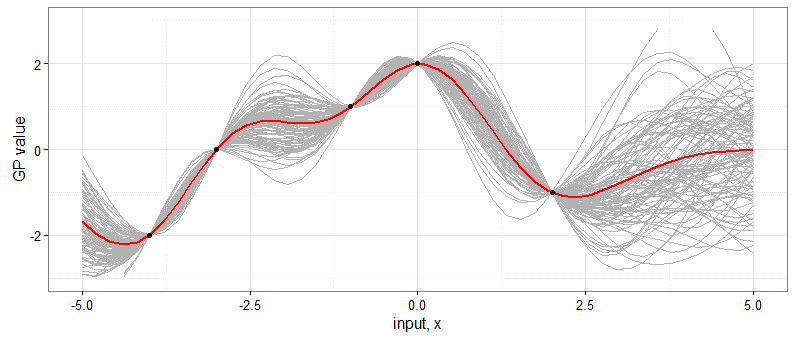
\includegraphics[width=.75\linewidth]{gp_example}
\caption{Example of a Gaussian process trained to interpolate five data points (black dots). The posterior mean function is shown in red; the gray lines are 50 draws from the posterior GP.}
\label{fig:gp_example}
\end{figure}

Though the approach of \cite{OHagan1978} was Bayesian, it did not provide for Bayesian means of selecting a covariance function $C$. \cite{Neal} extends the work of O'Hagan in this direction. \cite{Savitsky2011} describes a method for variable selection in GP regression via spike-and-slab mixture priors on the parameters of the covariance function. \cite{Shang2013} provide an umbrella generalization of existing methods of GP regression under a framework of what they call generalized GP models. All of these works treat GP regression generally, and do not focus specifically on the use of GPs to build emulators for computer model.

By contrast, much recent attention following the work of \cite{Santner2003a} and \cite{Sacks1989} has focused specifically on the use of GPs for computer model emulation. 
\cite{Kennedy2001} themselves develop an influential framework for Bayesian analysis using GPs specifically for computer model calibration. \cite{Kennedy2006} showcase this use of GP emulators for uncertainty and sensitivity analyses. \cite{Bastos2009} describes both numerical and graphical diagnostic techniques for assessing when a GP emulator of a computer model is successful, as well as discussion of likely causes of poor diagnostic results. While most work in the area of GP emulation uses stationary covariance functions (in which $C(x,y)=C(|x-y|)$ depends only on the distance between $x$ and $y$, and not on their location in the input domain) and quantitative inputs, efforts have been made to branch away from these core uses. \cite{Gramacy2008} use treed partitioning to deal with a nonstationary computer model. \cite{Qian2008} explore methods for using GP emulators that include both quantitative and qualitative inputs.

%\paragraph{Gaussian processes in computer model calibration}

Aside from \cite{Kennedy2001}, recent applications of GP emulation specifically to problems of calibration have focused largely on the works of \cite{Williams2006} and \cite{Bayarri2007}. It will be helpful here to provide an illustrative summary of the approach taken by \cite{Williams2006}, both to exemplify the use of GPs for computer model calibration and because the approach utilized in the present work closely follows theirs.

Consider that we have inputs $x\in \mathbb R^p$ and $t\in\mathbb R^q$ scaled to the unit hypercube, and observations 
\begin{equation}\label{eq:2}
y(x_i) = f(x_i) + \epsilon(x_i),\quad i=1,\cdots,n,
\end{equation}
where $f(\cdot)$ is the true system and $\epsilon(x_i)$ is known measurement error. Then by Equation \ref{eq:model_gen} we have
\begin{equation}\label{eq:2}
y(x_i) = \eta(x_i,\theta) + \delta(x_i) + \epsilon(x_i),\quad i=1,\cdots,n
\end{equation}
where $\eta(\cdot,\cdot)$ is the computer model, $\theta$ is the best\footnote{In the case of calibration, the ``best'' setting will be the true setting of that parameter; in a case of tuning rather than calibration, the ``best'' setting would instead be the optimal setting for minimizing model bias.}
setting of the vector of calibration parameters, and $\delta(\cdot)$ is the discrepancy function describing the bias of $\eta(\cdot,\cdot)$ as an estimate of $f(\cdot)$.

\citeauthor*{Williams2006} define the GP prior for modeling $\eta(\cdot,\cdot)$ as follows. Let the mean function $\mu(x,t)=c$, $c$ a constant. Set the covariance function to have the (stationary) form 
\begin{equation}\label{eq:Hig_cov}
C((x,t),(x',t')) = \frac 1\lambda_\eta \prod_{k=1}^{p}
\exp \left(-\beta^\eta_k|x_k-x_k'|^{\alpha_\eta}\right) \times
\prod_{k=p+1}^{p+q}
\exp \left(-\beta^\eta_{k}|t_k-t_k'|^{\alpha_\eta}\right)
\end{equation}
where $\lambda_\eta$ is the marginal precision of the GP; each $\beta_k$ describes the strength of the GP's dependence on one of the elements of the input vectors $x,t$; and $\alpha_\eta$ describes the smoothness of the GP. 

The authors place the following priors on the hyperparameter:
\begin{align}
\pi (c) &\sim N(0,v)\\
\pi(\lambda_\eta) &\sim \mathrm{Gamma}(5,5),\quad\lambda_\eta>0\\
\pi\left(\rho_k^\eta\right) &\sim \mathrm{Beta}(1,0.1),\quad k=1,\cdots,p+q
\end{align}
where $\rho_k^\eta=\exp(-\beta_k^\eta/4)$ $\forall k$. The parameters of the Gamma and Beta distributions are chosen to encourage $\lambda_\eta$ to be close to one, and $\beta_k$ to be low for all $k$ (encouraging strong dependence; i.e., we antecedently expect each of our inputs to be influential). Furthermore, the authors let $v\to0$, i.e., the GP is assumed to have constant mean $c=0$.

The authors similarly model the discrepancy term as a GP, also with mean zero, and covariance function
\begin{equation}
C_\delta(x,x') = \frac 1{\lambda_\delta} \prod_{k=1}^p
\exp\left( -\beta_k^\delta |x_k-x_k'|^{\alpha_\delta} \right),
\end{equation}
with priors
\begin{align}
\pi(\lambda_\delta) &\sim \mathrm{Gamma}(a_\delta,b_\delta)\\
\pi(\rho^\delta_k) &\sim \mathrm{Beta}(1,0.3).
\end{align}
where $\rho_k^\delta=\exp(-\beta_k^\delta/4)$ $\forall k$.

Then where $\boldsymbol \eta = (\eta(x_1,t_1),\cdots,\eta(x_n,t_n))^T$ are the simulation observations, $\mathbf y = (y(x_{n+1}),\cdots,y(x_{n+m}))^T= (y(x_{n+1},\theta),\cdots,y(x_{n+m},\theta))^T$ are the field observations, $\mathcal D = (\mathbf y^T \boldsymbol \eta^T)^T$, $\boldsymbol \beta^\eta = (\beta^\eta_1,\cdots,\beta_{p+q}^\eta)^T$, and $\boldsymbol \beta^\delta = (\beta^\delta_1,\cdots,\beta_{p+q}^\delta)^T$, we have the distribution of $\mathcal D$ as
\begin{equation}
\mathcal D | \theta,c,\lambda_\eta, \beta^\eta,\lambda_\delta,\beta^\delta,\mathbf C_y \sim N(c \cdot \mathbf 1_{n+m}, \mathbf C_{\mathcal D})
\end{equation}
where $\mathbf C_y$ an $m\times m$ matrix in which the $i,j$ entry is the (known) observation variance $C_{obs}(x_i,x_j)$ for $n<i,j\leq n+m$, and $\mathbf C_{\mathcal D}$ is a matrix with its $i,j$ entry equal to
\begin{equation}
C((x_i,t_i),(x_j,t_j)) + I(i,j>n)\cdot(C_{obs}(x_i,x_j) + C_\delta(x_i,x_j))
\end{equation}
Thus, the joint posterior density given by the model is
\begin{equation} \label{eq:full_dist}
\pi(\theta,c,\lambda_\eta,\rho^\eta,\lambda_\delta,\rho^\delta,\sigma^2|\mathcal D)
\propto \pi(\mathcal D | \theta,c,\lambda_\eta, \beta^\eta,\lambda_\delta,\beta^\delta,\mathbf C_y) \times \pi(c) \times \pi(\lambda_\eta) \times 
\pi(\rho^\eta) \times \pi(\lambda_\delta) \times \pi(\rho^\delta)
\end{equation}
where $\sigma^2$ gives the observation variance of the measurement error $\epsilon$. Note that where a discrepancy function is not included in the model and the mean $c$ is treated as a constant, (\ref{eq:full_dist}) simplifies greatly; where furthermore $\lambda_\eta$ and $\rho^\eta$ are estimated via maximum likelihood (as in  \cite{Kennedy2001}),  (\ref{eq:full_dist}) simplifies down merely to 
$\pi(\mathcal D | \theta,c,\lambda_\eta, \beta^\eta,\lambda_\delta,\beta^\delta,\mathbf C_y)$. Markov chain Monte Carlo methods are useful for evaluating (\ref{eq:full_dist}); the next section takes up this topic.

\subsubsection{Markov chain Monte Carlo methods}

%\paragraph{Background}

The central idea of Markov chain Monte Carlo (MCMC) integration is to construct a Markov chain which has as its equilibrium distribution the target distribution one wishes to explore. The Markov chain is observed, and beyond an initial ``burn-in'' period during which the chain is allowed to approach its equilibrium distribution, samples are considered to be drawn approximately from the target distribution.

For example, consider a model with full distribution given by (\ref{eq:full_dist}), but where discrepancy is not included and $\lambda_\eta,\rho^\eta$ are found via maximum likelihood estimation. Then the full distribution is given by $\pi(\theta,c,\lambda_\eta,\rho^\eta,\lambda_\delta,\rho^\delta|\mathcal D)
\propto \pi(\mathcal D | \theta,c,\lambda_\eta, \beta^\eta,\lambda_\delta,\beta^\delta,\mathbf C_y) \times \pi(c)$. A simple means of exploring this distribution via MCMC would begin with an initial guess $\theta^{(1)},c^{(1)}$. At the $i^{\text{th} }$ step for $i=2,\cdots$, using a proposal distribution $\pi_{prop}(\cdot,\cdot|{\theta^{(i-1)},c^{(i-1)}})$ from which we may easily sample directly, we draw a new ``proposed'' sample $\theta^*,c^*$. We then with probability $\alpha$ accept this new proposed sample, setting $(\theta^{(i)},c^{(i)}) = (\theta^*,c^*)$; otherwise we reject the proposed sample and let $(\theta^{(i)},c^{(i)}) = (\theta^{(i-1)},c^{(i-1)})$. In doing so, we have 
\begin{equation}\label{eq:mh-acceptance}
\alpha = \frac{\pi(\theta^*,c^* | \mathcal D)}{ \pi(\theta^{(i-1)},c^{(i-1)}|\mathcal D) } = 
\frac{ \pi(\mathcal D | \theta^*,c^*,\lambda_\eta, \beta^\eta,\lambda_\delta,\beta^\delta,\mathbf C_y) \times \pi(c^*)}{\pi(\mathcal D | \theta^{(i-1)},c^{(i-1)},\lambda_\eta, \beta^\eta,\lambda_\delta,\beta^\delta,\mathbf C_y) \times \pi(c^{(i-1)})}
\end{equation}
Note that in order to proceed in this way, it is necessary that $\pi_{prop}$ be a symmetric distribution. The version of MCMC described in this example is known as the Metropolis-Hastings algorithm; it was initially described by \cite{Metropolis1953} and generalized by \cite{Hastings1970}. A thorough exposition of the technique, its theoretical foundation, and its relation to other  varieties of MCMC is provided by \cite{Chib1995}.

% Gibbs
A related variant of MCMC -- in fact, a special case of Metropolis-Hastings, as shown by \cite{Gelman1992} -- is Gibbs sampling, initially described by \cite{Geman1984}. In using Gibbs sampling, one finds the conditional distribution of each of the parameters one wishes to sample, using the most recent samples of all other parameters. For example, we can convert the above Metropolis-Hastings illustration to a simple case of Gibbs sampling as follows.
Begin as before, with initial guesses $\theta^{(1)}$ and $c^{(1)}$. Thereafter, sample $\theta$ and $c$ not together, but rather in alternating draws. That is, at the $i^{\text{th} }$ step for $i=2,\cdots$, draw $\theta^{(i)}$ conditional on $c=c^{(i-1)}$, then draw $c^{(i)}$ conditional on $\theta=\theta^{(i)}$. Thus, for example, when drawing $c^{(i)}$, its conditional distribution would be proportional to $\pi(\mathcal D | \theta^{(i)},c^{*},\lambda_\eta, \beta^\eta,\lambda_\delta,\beta^\delta,\mathbf C_y) \times \pi(c^{*})$. 
If the conditional distribution is something from which we may easily draw directly, then we can draw $c^{(i)}$ that way; otherwise, we can use a so-called Metropolis-within-Gibbs scheme, and draw $c^{(i)}$ similarly to what was described above for the Metropolis-Hastings algorithm: draw a proposed $c^*$ from a proposal distribution, find the appropriate ratio $\alpha_c$, and accept or reject $c^*$ accordingly. In the application considered in the present work, Metropolis-within-Gibbs will be used.

%\paragraph{Elimination of boundary constraints}

Recall that a symmetric proposal distribution is required in order for the Metropolis-Hastings algorithm to proceed as described in the above illustration of that technique. However, the algorithm can accommodate an asymmetric proposal distribution with only slight complication. A frequent reason for using an asymmetric proposal distribution is the existence of boundary constraints on the parameter being sampled. Thus, for example, in the application considered in the present work, one of the calibration parameters is the thickness (in mm) of the material forming a wind turbine blade. Expert opinion was used to set the support of this parameter to be the range [10mm, 25mm]. Good mixing in the MCMC chain is promoted by choosing a proposal density such that the distribution $\pi_{prop}(\cdot|\tau)$ has mean $\tau$. With boundary constraints, this requires an asymmetric distribution. When $\pi_{prop}(\cdot|\tau)$ is asymmetric, this changes the above illustration only by way of requiring us to calculate the acceptance probability $\alpha$ as follows:
\begin{equation}\label{eq:mh_correction}
\alpha = \frac{\pi(\theta^*,c^* | \mathcal D)}
{ \pi(\theta^{(i-1)},c^{(i-1)}|\mathcal D) } \times 
\frac{
\pi_{prop}(\theta^{(i-1)},c^{(i-1)}|\theta^*,c^*)
}{
\pi_{prop}(\theta^*,c^*|\theta^{(i-1)},c^{(i-1)})
}.
\end{equation}

%\subsubsection{Normalization of inputs and standardization of outputs}
%Blah

\subsubsection{Computational difficulties}
% And solutions
Note that the joint posterior density given in (\ref{eq:full_dist}) above includes $\mathbf C_{\mathcal D}$, which, depending on how many field and simulation observations one has, may be of fearsomely high dimension. This can lead to computational difficulties in calculating $\alpha$ in the course of the MCMC routine. Difficulties arise in two ways. Firstly, the likelihood given in (\ref{eq:full_dist}) evaluated at a given point can be so small as to be vulnerable to significant round-off error. Secondly, the poor conditioning of $\mathbf C_{x,x}$ in (\ref{eq:post_gp}) can make it difficult to invert and find the determinant of this matrix, as must be done in the course of the MCMC to find the relevant likelihoods. The latter problem can be alleviated by adding a small nugget to $\mathbf C_{x,x}$; i.e., (abusing notation somewhat) we can set $\mathbf C_{x,x}= \mathbf C_{x,x} + \xi \cdot \mathbf I_{\mathrm{dim}(\mathbf x)}$ for some very small value of $\xi$, e.g., $\xi=10^{-4}$. For a more sophisticated way of selecting the nugget size, see \cite{XXX}. Note that adding a nugget here is equivalent to adding a small amount of observation variance for the simulator observations. That is, in adding this nugget, we no longer require that the GP emulator precisely interpolate the simulation observations. However, for very small nuggets, this effect is so small as to be insignificant, though the computational benefits remain. Thus nothing is lost in continuing to think of the GP emulator as interpolating the simulation observations.

The other problem -- round-off error due to small likelihoods -- can be alleviated through substituting the use of log-likelihoods in the MCMC routine. Thus, rather than finding $\alpha$ in (\ref{eq:mh_correction} directly, it is preferable to find 
\begin{equation}\label{eq:log_lik_alpha}
\log \alpha = \log \pi(\theta^*\!,c^* | \mathcal D) + \log \pi_{prop}(\theta^{(i-1)}\!,c^{(i-1)}|\theta^*\!,c^*) - \log \pi(\theta^{(i-1)}\!,c^{(i-1)}|\mathcal D) - \log \pi_{prop}(\theta^*\!,c^*|\theta^{(i-1)}\!,c^{(i-1)})
\end{equation}
Of course, in order to enjoy the computational benefits of this approach, one must perform calculations on the log scale from the start; it would not do to, e.g., find $\pi(\theta^*, c^*|\mathcal D)$ on its original scale and then take its log. 

\section{Calibration for design}\label{calib_for_design}

% Intro: description of sort of situation in which you'd want this

Suppose that a researcher has a fairly reliable computer model of a given system. Suppose furthermore that some of the parameters of that system can be controlled, and that the researcher hopes to select values for these controllable parameters that will facilitate certain target outcomes from the system. An example would be selecting a building layout conducive to efficient evacuation, as modeled using SIMULEX.

We may approach such problems as a matter of calibration. In traditional calibration as described in Section \ref{introduction}, a computer model is calibrated to observations of reality. This is done in order to find settings for the computer model that induce its output to match reality. Similarly, one may seek to ``calibrate'' a computer model to a set of \emph{desired} observations, in order to find settings that induce the model's output to match those desires. 

Of course, computer models are more malleable than reality, and it is trivial to modify a computer model so that its output matches any given target; there is little difficulty and less value to creating a computational ``yes man''. But in many cases one is fortunate to have (perhaps after undertaking traditional model calibration, validation and verification) a computer model such that one is independently confident of the model's faithfulness to reality over a given range $\mathcal T$ of controllable parameters $t$. In such a circumstance, in calibrating $t\in\mathcal T$ to one's desires, one does not risk calibrating the model \emph{away} from agreement with reality; instead, one finds the settings that achieve the best realistic approximation to the desired observations.

The tools of model calibration founded in the work of \cite{Kennedy2001} retain their advantages in this new domain. Most centrally, such calibration to desired observations $y$ produces not merely a static optimum $t\in\mathcal T$, but rather a posterior distribution of $t|y$ reflective of remaining uncertainty about the appropriate value of $t$. Such uncertainty may have its source in parameter uncertainty (uncertainty about the values of certain model inputs), code uncertainty (uncertainty about how closely the code approximates reality), and especially saliently in this case, what in traditional calibration would be considered either observation error or model inadequacy. Of course, our desired observations are not actually observations, and the concept of observation error does not cleanly transfer here. But a relevantly similar uncertainty would be uncertainty over how close reality \emph{can} come to our desired observations. The model calibration framework of \cite{Kennedy2001} allows for the quantification of all of these uncertainties.

\subsection{Desired observations}
% This describes the basic idea.
% Include discussion: how do we select desired data?
% Also include discussion of how this is actually effected. This discussion will be short, because the answer is that it will use the framework described already in the previous section.


\subsubsection{Level of desired data}
% Arbitrariness recommending prior on observation variance
Unlike in the case of field observations, when calibrating to desired observations, the question arises of determining what exactly one's desired observations are. In many cases, no objectively natural target manifests itself. Consider again the case of building evacuation. In the case of a multi-story building, one might plausibly expect to achieve evacuation times of no less than fifteen minutes. But plausibility is no barrier to desire, and it would be a mistake to limit one's desired observations to what is antecedently believed to be achievable, if only because to do so would foreclose on the possibility of exceeding those expectations. In the case of building evacuation, then, one might conclude that the desired observation is in fact instantaneous evacuation -- \textit{per impossible}. But, having discarded realism, even this lower bound is not inevitable. Why not calibrate to a \emph{negative} evacuation time, while we're at it?

Such a choice of desired observation would indeed be consistent with the method of calibrating to desired observations, and in certain situations may even be appropriate. However, in general, desired observations should aim only a little beyond what is realistically achievable. I described above why it is preferable to go beyond what is achievable. There are two reasons why one should go only a little beyond that. (1) If desired observations are set to be too farfetched, then the relevant likelihoods can become unnecessarily computationally unstable due to underflow and round-off error. (2) The desired observations lose a measure of interpretability when they delve too far into the fantastical, such as with negative evacuation times. Identifying the appropriate range of outputs for desired observations, which exceed reality but slightly, will of course often require one to consult expert opinion. 

\subsubsection{Set target via desired data, or prior distribution?}

In undertaking model calibration to achieve desired system output, directly setting desired observation is not the only option. For example, in the application considered below in Section \ref{application}, the calibration parameters are controllable features of material design, and the cost of the resulting material is one of the outputs for which we establish targets. Two approaches are used for doing this. One approach is simply to include a desired observation of cost, and calibrate to that along with the other desired observation targets. The alternative approach is to remove cost from the model, and set a prior over the remaining calibration parameters such places low probability over those regions of $\mathcal T_{-c}$ (the calibration parameter space excluding the cost dimension) for which the cost is high. Of course, this requires broad prior knowledge of the behavior of cost over $\mathcal T_{-c}$; without such knowledge, this alternative would be unavailable.

A third option is also explored in Section (\ref{application})'s treatment of the material design application. This option is not truly another means of achieving a calibration target, but rather is simply the decision to refrain from doing so. That is, rather than include a desired observation of (e.g.) cost in the above model or set a prior that induces low cost, we can simply specify a known cost and calibrate desired performance targets for a design having that cost. Since we are antecedently ignorant of which cost settings are optimal, under this third option we calibrate performance targets under each point of a grid of ``known'' costs. Thus we achieve a comprehensive picture of optimal parameter distributions and resulting performance under a range of costs, which could inform the process of setting a budget for material construction.

\subsection{Model shortcoming}
% How do we account for the model's failure to achieve our desired data?
% Through observation variance quote unquote?
% Or through the discrepancy function.
% The is a way of letting the errors be correlated, which may be nice

Note that it is not merely likely but often desirable that the desired observations have low likelihood with respect to the posterior predictive distribution of the calibration process. This is another way in which calibration to desired observations is unlike traditional calibration. The reason for this is that if the posterior predictive distribution places substantial probability mass at regions of the parameters space that achieve the target desired observations, then this is a sign that the the desired observations may have been insufficiently ambitious. 

In some applications, this concern will not arise. In general, this concern applies whenever one's desired output from a system is not limited to what is realistically achievable. In the building design example, we would like to see instantaneous evacuation; in the material design case, we would like to see zero-cost materials that do not deform at all under load. These targets are unattainable, but we wish to induce the system to approach these targets, and so these impossibilities become our desired observations. However, another type of calibration to desired observation may involve searching within the space of what is achievable. In a different application than the one considered in this work (wind turbine blades), it might be ideal to have a material that deforms just so -- rather than a material which does not deform under load. In such a case, it would be appropriate to set desired observations that one hopes to find as the posterior predictive mode after calibration. But in cases such as the wind turbine and building evacuation systems, finding the desired observations to be the posterior mode would be an indication that the desired observation could potentially be outperformed, or else that the model is itself unrealistic. In short, if the system can achieve the desired observations, then either the desired observations are realistically achievable (hence insufficiently ambitious) or else the desired observations are not realistically achievable (hence casting doubt on a model which presents them as achievable).

Where the mean of the posterior GP from calibration to desired observations fails to interpolate those desired observations, this can be understood in two distinct ways. These correspond to the two distinct sources of error in traditional calibration to field observations. The first such source of error is model discrepancy, or $\delta(\cdot)$ in (\ref{eq:model_gen}). This is defined to be the difference between the mean of the true system and the output of the computer model; it is thus the extent to which the computer model fails to capture reality. The other source of error is observation error, or $\epsilon(\cdot)$ in (\ref{eq:model_gen}). This is irreducible error, usually taken so that $\epsilon(x) = \epsilon$ is independent of $x$. Note that this source of error cannot be attributed to any failing on the part of the computer model. Neither of these two sources of error, under their above-described traditional interpretations, succeeds in capturing the nature of the gap between desired observations and the posterior predictive mean. These two sources of error can nonetheless serve as a basis for modeling this gap -- see (\ref{obs_error}) and (\ref{mod_disc}) below.

Nor does it quite fit even to call this gap ``error'', or a form of model discrepancy. Even under calibration to desired observations, the model still describes \emph{reality}, not our desires. Thus failure to interpolate our desires is not error. Though for convenience and ease of exposition I will often slip back into referring to this gap as ``error'', we can more properly refer to it as ``model shortcoming''. This is still somewhat infelicitous insofar as it still implies failure on the part of the model, whereas in fact this gap is due to the stubbornness of \emph{reality} in declining to behave according to our desires\footnote{Though maybe a more enlightened viewpoint would take a conflict between reality and desire to be the latter's fault.}. The model underperforms with respect to our targets insofar as reality does so. Still, the term is appropriate, since the ``error'' observed is a discrepancy between the desired observations and the model, not between the desired observations and the true system.

\subsubsection{Observation error}\label{obs_error}

% Specifying observation error (including specifying different errors)

% Setting a prior on observation error

Model shortcoming can most straightforwardly be accommodated by treating it as observation error $\epsilon(\cdot)$. This approach is flexible and has a number of advantages.

Firstly, this approach allows one to specify ``known'' observation variance. In the framework of calibration to desired observations, this amounts to specifying how strongly the posterior GP should be drawn to the desired observations. This would be especially useful in the sort of case, described above, in which one hopes the posterior GP to (nearly or precisely) interpolate the desired data. Even in the more ambitious sort of case when the desired observations are realistically unattainable, there is great flexibility to be exercised in selecting observation variances directly. One can thereby, for example, set priorities in one's targets. For example, in the application of Section \ref{application}, there are three outputs: wind turbine blade tip deflection, rotation, and cost. A plausible scenario for design would be that keeping costs low might be a much greater priority than minimizing deflection and rotation. This can be achieved simply by setting the observation variance of cost to be lower than that of deflection and rotation. This approach is amongst those implemented in Section \ref{application}.

However, one might antecedently have little information about just how close the model can come to the desired observations. This is especially true when multivariate output is considered. The model may be able to approach some elements of the desired observation much more closely than others. Without prior knowledge, it can thus be difficult to specify an appropriate setting for the observation variance. Too low, and computational difficulties may arise from low likelihoods. Too high, and the model may be insufficiently ``incentivized'' to approach the targets. In such situations, one can simply place a prior on the observation variances, allowing the simulation observation data to inform us as to how achievable the desired observations are. In Section \ref{application} I implement this, showing that it leads to more successful MCMC and better performance with respect to the desired observations than specifying a static observation variance.

Finally, these two methods can be combined. One of the approaches used in Section \ref{application} places a prior over the observation variance of deflection and rotation, but specifies a very low observation variance for cost, over a grid of (realistically achievable) desired cost observations, each of which is paired with (unrealistically ambitious) desired observations of zero deflection and rotation. The net result of this is to find distributions of optimally performing materials over a grid of set costs, so that one can see the performance outcomes as variables of a choice of cost over a broad range.

%Thus, the use of observation variance to incorporate model shortcoming is a flexible approach that can accommodate a variety of different calibration problems. The primary disadvantage of this approach to model shortcoming is its interpretability. 

\subsubsection{Model discrepancy}\label{mod_disc}

A separate means of incorporating model shortcoming would be to treat it as model discrepancy $\delta(\cdot)$ rather than as observation variance. Ordinarily, $\delta(\cdot)$ is itself modeled as a mean-zero GP; see (\ref{gaussian_processes}) above. This has the advantage that it facilitates treating model shortcoming as correlated, which will typically be the case; the deviance of our desired observations from the mean is after all not mere Gaussian noise.

Disadvantages are that in contrast with the use of observation variance, it is much less convenient to fine-tune the model discrepancy function to the details and priorities of a particular situation. For example, like \cite{Williams2006}, we use dummy variables to construct a univariate Gaussian emulator for our three model outputs; the dummy variables serve to differentiate the three outputs. If we now wish to either specify different variances for the three outputs or to allow the data to discover different such variances (as suggested above for observation variances) via a model discrepancy function, we will not be able to use a stationary GP to model that discrepancy. That is, the covariance function for the discrepancy GP, $C_\delta(x,x')$, will depend not only on the distance between $x$ and $x'$, but on their location within the input space $\mathcal X$. This is an unattractive complication, but remains a live option.

\subsection{Field observations and model discrepancy}
% Here, discuss whether or how to include field observations.

In the version of model calibration to desired observations presented thus far, the calibration has been entirely to desired observations. This invites the question of how to proceed when one wants to undertake both traditional calibration and calibration to desired observations. In other words: what happens when we have both desired observations \emph{and} field observations? 

It may be tempting to undertake both calibrations simultaneously; however, this will typically not be possible. The reason is that these two sorts of calibration parameters tend not to overlap in the matter of which parameters are considered to be calibration parameters. The purpose of calibration to desired observations is to find optimal settings for parameters over which we have control; it's no use finding out that (e.g.) a building will be most efficiently evacuated when the occupants have average walking speed $s$, since we have no power to mandate the average walking speed of people fleeing a burning building. Instead, given a distribution on walking speeds, we may seek to find the layout that best contributes to efficient evacuation; the building layout is under our control. By contrast, in traditional calibration, one ordinarily specifically calibrates those parameters over which we have no control, and whose true value we seek to discover. Thus, using field data from building evacuations, a researcher might use traditional calibration to try to calibrate SIMULEX to the appropriate distribution on walking speeds -- there treating building layout to be fixed (as the layout(s) of whichever buildings were evacuated in the field observations).

Thus to simultaneously undertake traditional calibration and calibration to desired observations, where the calibration and control parameters of each of those two calibrations are not aligned, is not possible under the framework of \cite{Kennedy2001}. Instead, the most obvious solution is to undertake traditional calibration prior to calibration to desired observations, finding both a distribution on the (traditional) calibration parameters and an estimated model discrepancy function. Thus one arrives at the calibration to desired observations (assuming success in the former calibration) with a model that faithfully represents the true system.

In the unlikely event that the calibration parameters coincide under the two sorts of calibration, it would be possible to undertake a single round of calibration to both field and desired observations. It would be necessary to take care with how to treat model shortcoming in this scenario. Attempting to capture it via the model discrepancy function would likely lead to confounding the true model discrepancy with the model shortcoming, undermining both calibration goals. A more hopeful route would be to use observation variance to incorporate the model shortcoming; this would allow one to specify a larger observation variance for desired observations than for field observations (and that only if these two sets of observations do not share locations in $\mathcal X$). Even this strategy would only mitigate the confounding of the two calibration goals, and should only be used if the budget for simulation observations is so small as to make it infeasible to perform two separate calibrations.

\subsection{Hyperparameter estimation}\label{hyperparameter_estimation}
% Basically, make the case for modularization here. So your desired data doesn't infect your hyperparameters. After all, you want these set to most closely emulate the computer model. You want these reflecting reality, not reflecting your targets.
Consider the covariance function parameters $\lambda_\eta,\beta^\eta$ of (\ref{eq:Hig_cov}). In a full Bayesian analysis, these would be searched over in the MCMC along with the calibration parameters. However, \cite{Kennedy2001} instead find the MLEs of these hyperparameters prior to calibration. More generally, \cite{Liu2009} advocate modularization, described in Section \ref{computer_model_calibration} above. A key motivation of modularization is to protect good components of the model from ``suspect'' components of the model, and desired observations are, by their very nature, ``suspect''. In other words, the model most successfully represents reality when the settings for these hyperparameters are guided by accurate and precise information about the true system. Desired observations are deliberately not such information. In essence, attempting a full Bayesian analysis that finds these hyperparameter settings as part of the calibration to desired observations would be committing the same sort of error as described in the previous section: namely, calibration to desired observations should be used to tune only those parameters which are within our control over a range $\mathcal T$ such that the model faithfully represents reality over all of $\mathcal T$. In the true system, the hyperparameters of the covariance function are not under our control.

Therefore, care should be taken to prevent the infection of covariance hyperparameters by the desired observations. The way that this is accomplished in the application of Section \ref{application} is to use maximum likelihood estimation from the simulation observations alone to estimate these values. Field observations could be used here as well, either for the maximum likelihood estimation or for a modular Bayesian analysis \`a la \cite{Liu2009}.

\section{Application}\label{application}

In this section I apply calibration to desired observations to the problem of selecting a material for constructing a wind turbine blade of fixed geometry. In traditional engineering design, material selection is a matter of selecting a material with appropriate properties for the project at hand from a database of known materials, often as a matter of ad-hoc satisficing. Material design usually occurs separately, and without an eye to specific end-uses. It is desirable to wed these design processes, selecting a material design by modeling its performance outcomes in a particular engineering application. Therefore, here I offer a calibration of material design parameters to desired performance targets for a wind turbine blade. This calibration is mediated by a finite element model using \texttt{ANSYS} simulation software\footnote{
The finite element code was authored by Evan Chodora.
}
, which is treated as an unbiased representation of reality.

\subsection{Project background}

Two primary performance targets for the design and construction of wind turbine blades is the distance (in meters) that the blade tip deflects under load from its starting position, and the angle (in radians) that the blade undergoes rotation when under load. Each of these measures should ideally be as close to zero as possible. In selecting the composite material used to build the turbine blade, given a choice of matrix and filler materials, the properties of the material depend on the \textit{volume fraction} -- the volume ratio of filler material to matrix material used in the composite -- and the thickness of the material used to build the blade. The resulting material properties impact the performance of the blade, as well as its cost per square meter. 

The finite element model takes as inputs a triplet $(t,v,k)$, which are respectively the operating temperature of the wind turbine (in kelvin), the volume fraction of the material, and the thickness of the material. The outputs of the model are a triplet $(d,r,c)$, which are tip deflection (in meters), rotation (in radians), and cost per square meter (USD). The wind turbine should be capable of operating over the range of temperatures 230K-330K. The goal of calibration is thus to find posterior distributions on $v$ and $k$ given observations from the finite element simulator and desired observations.

\subsection{Emulation of finite element simulator}\label{emulator}
The finite element simulator is too computationally expensive to be suitable for direct use in (e.g.) an MCMC routine. Thus I employ a GP emulator in the manner of \cite{Williams2006}. For this purpose, 504 observations were drawn from the finite element simulator. These observations follows a LHS design based on plausible ranges for the three inputs, as identified by expert opinion.

We consider the finite element observations to be distributed as $\mathcal{GP}(0,C)$; that is, a GP with mean 0 and covariance function $C$ as described by (\ref{eq:Hig_cov}) above, with $\alpha_\eta=2$. We do not include a discrepancy function, per the considerations of Section \ref{obs_error}.

The hyperparameters $\lambda_\eta,\beta^\eta$ must be estimated. Per the considerations of Section \ref{hyperparameter_estimation}, we do not estimate these values as part of a full, integrated Bayesian analysis; instead, they are estimated prior to calibration to the desired observations, via maximum likelihood estimation. Initially, a grid optimization method was used: a grid of $\beta^\eta$ values was used, finding at each point of the grid the likelihood of the simulation observations integrated over the support of $\lambda_\eta$. However, $\beta^\eta$ is a five-dimensional vector, and a grid fine enough to be useful was too computationally burdensome to be feasible. Instead, a gradient descent method was used to maximize the log-likelihood of the simulation observations over the joint (6-dimensional) support of $\beta^\eta,\lambda_\eta$.  The result is given by
\begin{equation}\label{eq:MLEs}
\rho^\eta = (0.9358, 0.6509, 0.6736, 0.4797, 0.9673),\quad
\lambda_\eta = 0.0152
\end{equation}
where $\rho^\eta_k = \exp(-\beta_k^\eta/4)$. A slice of the resulting emulator mean (for thickness = 20mm) for the tip deflection output is shown in Figure \ref{fig:emulator_surface}.

%\subsubsection{Wind turbine blade simulator}
%% Here the finite element model will be described
%Blah
%
%\subsubsection{Mathematical basis for the emulator}
%% Includes formulae for trained mean and covariance functions
%Blah
%
%\subsubsection{Experimental design}
%% How we selected the design points at which to observe the simulator
%Blah
%
%\subsubsection{Covariance parameters}
%% How they were selected
%Blah

%\paragraph{Finding covariance parameters via MCMC}
%% Why we didn't do it (computational difficulties
%Blah
%
%\paragraph{Grid optimization}
%% Advantages and disadvantages; full grid and integration of lambda
%Blah
%
%\paragraph{Gradient method}
%% Explanation and advantages
%Blah

\begin{figure}
\centering
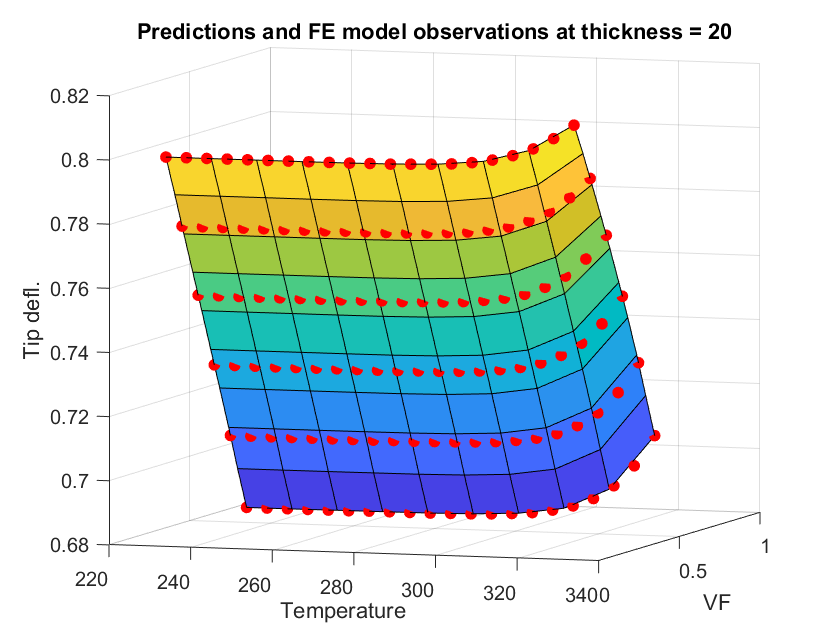
\includegraphics[width=.65\linewidth]{emulator_surface}
\caption{A slice of the GP emulator mean (restricted to the output for tip deflection) at thickness = 20mm. Red dots are observations from the simulator.}
\label{fig:emulator_surface}
\end{figure}

\section{MCMC using the emulator}\label{MCMC}

%\subsection{MCMC methods}
%% Background on MCMC
%Blah

\subsection{The model}
% Choice of priors and resulting likelihood
Following the framework laid out in Section \ref{gaussian_processes} and the hyperparameters estimated in Section \ref{emulator}, the model takes the trained emulator to be distributed as
\begin{equation}\label{posterior_GP}
\mathcal {GP}\left(\mu^*(z), C^*(z,z')\right)
\end{equation}
where $\mu^*(z) = \mathbf C_{z,\mathbf z} \cdot C_{\mathbf z,\mathbf z}^{-1} \cdot \boldsymbol \eta$, $C^*(z,z') = \mathbf C_{(z^T,z'^T)^T,(z^T,z'^T)^T} - \mathbf C_{(z^T,z'^T)^T,\mathbf z}\cdot \mathbf C_{\mathbf z,\mathbf z}^{-1} \cdot \mathbf C_{\mathbf z,(z^T,z'^T)^T}$, $\mathbf C_{a,b}$ is the matrix whose $i,j$ element is equal to the covariance between the $i^{\text{th}}$ row of $a$ and the $j^{\text{th}}$ row of $b$, $z=(x,t)$ is a row vector of control and calibration inputs, $\mathbf z=(z_1^T,z_2^T,\cdots,z_n^T)^T$ is the $1512\times5$ matrix of locations of the 1512 simulation observations, and $\boldsymbol\eta$ is a column vector of the 1512 simulation responses: $\boldsymbol\eta_i=\eta(\mathbf z_i)$. All model inputs are normalized to [0,1] over their supports; all model outputs are standardized so that $\boldsymbol\eta$ has mean 0 and standard deviation 1.

$C(\cdot,\cdot)$ is given by (\ref{eq:Hig_cov}) on page \pageref{eq:Hig_cov}, where we plug in the MLEs given in (\ref{eq:MLEs}). Generalizing from \cite{Kennedy2006}, we expand the Bayesian analysis to include the diagonal observation variance matrix $\mathbf C_y$, rather than requiring this value to be specified as known, and we allow for a non-uniform prior $\pi(\theta)$ on the calibration parameters. By (\ref{eq:full_dist}) on page \pageref{eq:full_dist}, 
since we estimate $\rho^\eta,\lambda_\eta$ by maximum likelihoods, set $c=0$ and do not include a discrepancy function, for desired observations $\mathbf y=(y (z_{n+1}),\cdots,y(z_{n+m}))^T$ and $\mathcal D=(y^T, \boldsymbol\eta^T)^T$ we have
\begin{equation}\label{eq:the_model}
\pi(\theta,\sigma^2) \propto \pi (\mathcal D|\theta,\mathbf C_y)\times \pi(\theta)\times \pi(\mathbf C_y)
\end{equation}
where $\mathcal D|\theta,\mathbf C_y \sim N(\boldsymbol 0_{m+n}, \mathbf C_{\mathcal D})$ with 
\begin{equation}\label{eq:the_covariance}
\mathbf C_{\mathcal D} = \mathbf C_{\boldsymbol\eta} + 
\begin{bmatrix}
\mathbf C_y & \boldsymbol 0\\ 
\boldsymbol 0 & \boldsymbol 0
\end{bmatrix}
\end{equation}
where $\mathbf C_{\boldsymbol\eta}$ is a $(m+n)\times(m+n)$ matrix with $i,j$ entry $C(z_i,z_j)$.

The model as described above leaves open several details of the model, options for which are explored in the remainder of Section \ref{MCMC}. In \ref{des_obs_var} we consider options for $\pi(\mathbf C_y)$, the prior on observation variance, including setting a degenerate prior corresponding to specifying a known observation variance. In \ref{which_data} we take up the question of which data one ought to desire, showing how the goals of one's analysis can support vastly different choices for desired data. In \ref{non-uniform_prior} we explore options for $\pi(\theta)$, the prior on observation variance. We depart thereby from the framework of \cite{Kennedy2006}, who (implicitly) restrict the calibration model to the case of using a uniform prior. An example is used to show how setting a non-uniform prior here can allow one to reduce the number of calibration parameters in the model. Before taking up these matters, in \ref{convergence_difficulties} we take up convergence difficulties that arise due to boundary constraints on the calibration parameters.
%\subsubsection{Full model and likelihood}
%Blah

\subsection{Convergence difficulties}\label{convergence_difficulties}
% And the idea to eliminate boundary constraints
As will often be the case in calibration problems, in the application considered here the calibration parameters $(v,k)$ have compact support: $v\in [.1,.6],$ $k\in [10\mathrm{mm},25\mathrm{mm}]$. When the calibration procedure leads to draws near these boundaries, the MCMC routine may suffer poor mixing. For example, consider using proposal density $\pi_{prop}$ such that $(v^*,k^*)\sim N((v^{(i)},k^{(i)}),\Sigma)$ (for some proposal covariance $\Sigma$). The symmetry of a normal proposal density makes it convenient for MCMC, but also exacerbates the difficulties that come from boundary conditions. Using such a proposal density with $\pi(\theta)$ a uniform density on the supports of $\theta$ amounts to simply discarding any proposed draw of $(v,k)$ that falls outside of the boundaries for those variables. This is inefficient, as it leads to low acceptance rates during MCMC for new draws of $\theta$. When a new proposed draw is rejected, the previous draw is repeated, leading to extremely high levels of autocorrelation in the MCMC draws.

This problem can be mitigated through utilizing an adaptive proposal covariance, so that $\Sigma$ is periodically updated during the burn-in period in order to achieve an optimal acceptance ratio of around 25\%; see \cite{Roberts1997}. If $\Sigma$ is diagonal, then this is especially simple to implement; one simply keeps track of the number of times that a proposed draw of $\theta_i$ is outside of its boundaries, and then every 100 MCMC steps or so, if the number of out-of-boundary proposals exceeds a specified threshold, then one reduces $\Sigma_i$, the proposal variance of $\theta_i$. This strategy can easily be paired with a more comprehensive adapative proposal covariance -- e.g., one that is set to increase in magnitude whenever more than 40 of the most recent 100 draws have been accepted, and decrease in magnitude whenever fewer than 15 of the most recent draws have been accepted.

If the posterior distribution is merely near the boundary, such measures may suffice; however, in calibration to desired observations (which tend to be extreme outliers \textit{qua} observations), often the calibration parameters will be drawn strongly to the boundaries, and in such a situation the sort of adaptive proposal distribution described above may be insufficient to secure good acceptance ratios. Here, some variety of non-symmetric proposal is likely to be of help.

In the case of compact support, 

\subsubsection{Implementation of the Metropolis-Hastings algorithm}
Blah

\begin{figure}
\centering
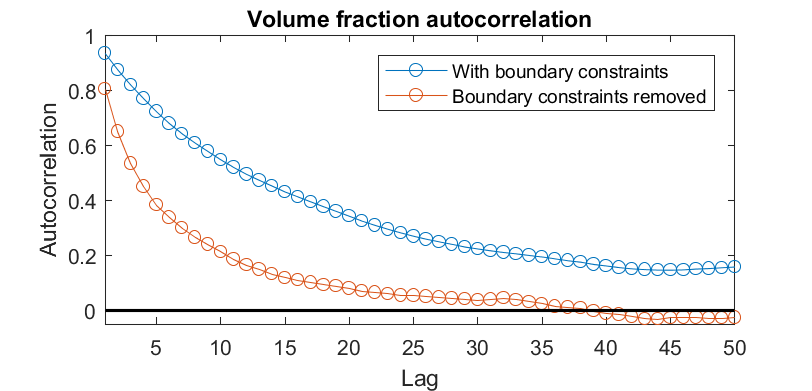
\includegraphics[width=.9\linewidth]{ACF_bnd_cnds_fig}
\caption{Auto-correlation for draws both with and without the elimination of boundary conditions.}
\end{figure}

\subsection{Desired observation variance}\label{des_obs_var}
% 4 versions: heterosked constant, homosked constant, heterosked prior, homosked prior
\begin{table}[h]
\centering
\begin{tabular}{| c | c  |  c  | c |  c  |}
\hline
 \vspace{-3mm}
& & & & \\
& \parbox{24mm}{\centering Heteroskedastic, constant}& \parbox{24mm}{\centering Homoskedastic, constant}& \parbox{24mm}{\centering Heteroskedastic, prior} & \parbox{24mm}{\centering Homoskedastic, prior}\\
 \vspace{-3.5mm}
& & & & \\
\hline
Deflection & 0.749 & 0.729 & 0.659 & 0.709\\
Rotation & 0.0904 & 0.0865 & 0.0773 & 0.0843\\
Cost & 276.16 & 236.11 & 350.80 & 233.95 \\
\hline
\end{tabular}
\caption{Comparison of model outputs, where the desired data outputs are assumed to be either homoskedastic or heteroskedastic, with either a specified constant variance or a $1/\sigma^2$ prior.}
\label{table:obs_var_comp}
\end{table}

\begin{figure}
\centering
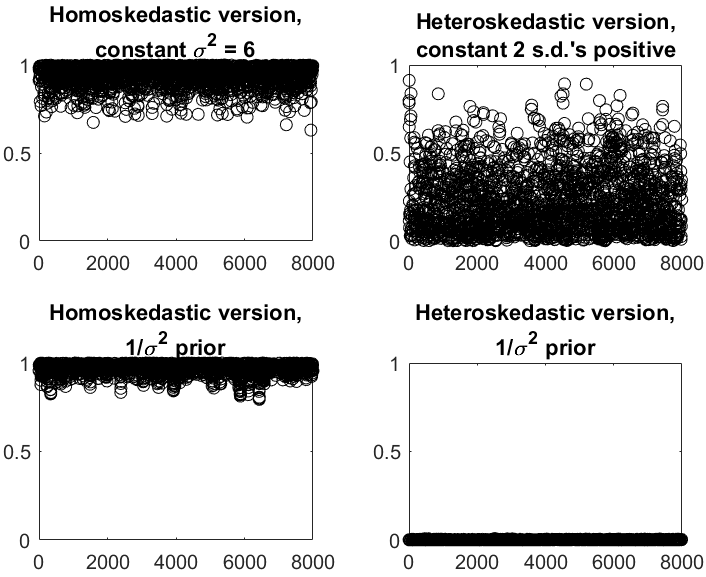
\includegraphics[width=.65\linewidth]{comp_obs_var}
\caption{MCMC results at various observation variance settings.}
\label{fig:comp_obs_var}
\end{figure}

\subsection{Which data to desire?}\label{which_data}
Blah

\subsubsection{Motivations behind the choice of desired data}
Blah

\subsubsection{Differing results}
% for different desired data values
\begin{table}[h]
\centering
\begin{tabular}{| c | c  | c  |  c | c  | c | c | c |}
\hline
Desired data $d$ & $\sigma^2_{defl}$ & $\sigma^2_{rot}$ & $\sigma^2_{cost}$ & $\mu_{v|d}$ &
                            $\mu_{h|d}$ & $\sigma^2_{v|d}$ & $\sigma^2_{h|d}$\\
\hline
$(0, 0, 0)$ & 375.45 & 277.69 & 2.62 & 0.215 & $4.01 \cdot 10^{-2}$&
	$4.41\cdot 10^{-2}$ & $1.92 \cdot 10^{-3}$\\
$(0.65, 0.077, 96)$ & 16.74 & 15.25 & $4.62 \cdot 10^{-7}$ &
	$1.09 \cdot 10^{-3}$ & $3.36 \cdot10^{-4}$ &
	$1.02 \cdot 10^{-5}$ & $9.97 \cdot 10^{-6}$\\
\hline
\end{tabular}
\caption{Comparison of results for two different (low) values of $d$. Values listed are, respectively, the posterior means for the observation variance of each model output, posterior means for volume fraction ($v$) and thickness ($h$), and posterior variance of volume fraction and thickness.}
\label{table:d_comp}
\end{table}

\begin{figure}
\centering
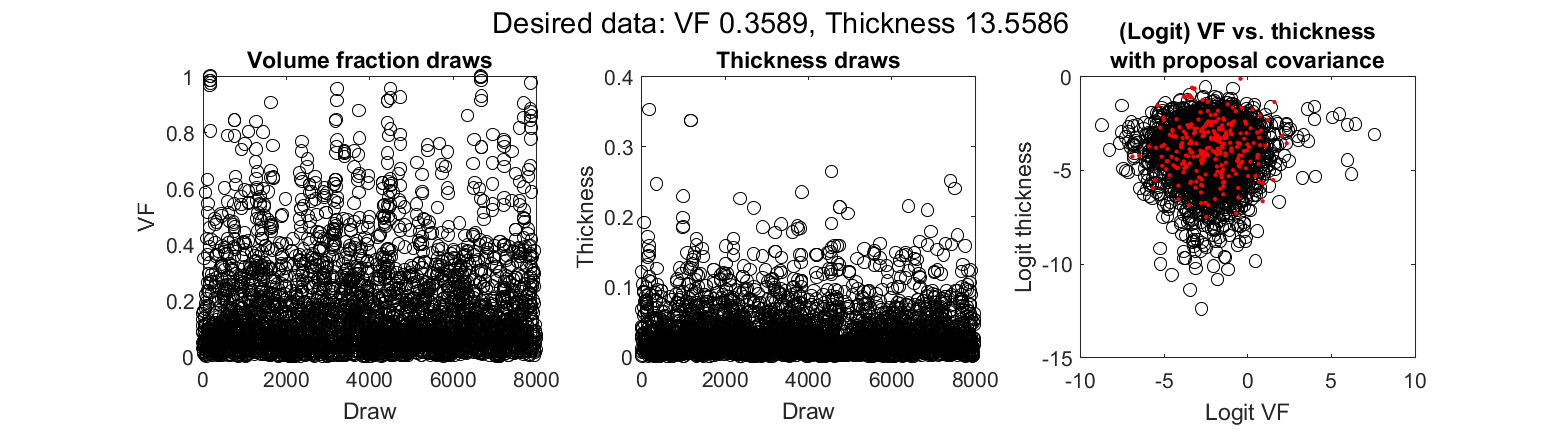
\includegraphics[width=.9\linewidth]{FIG1}
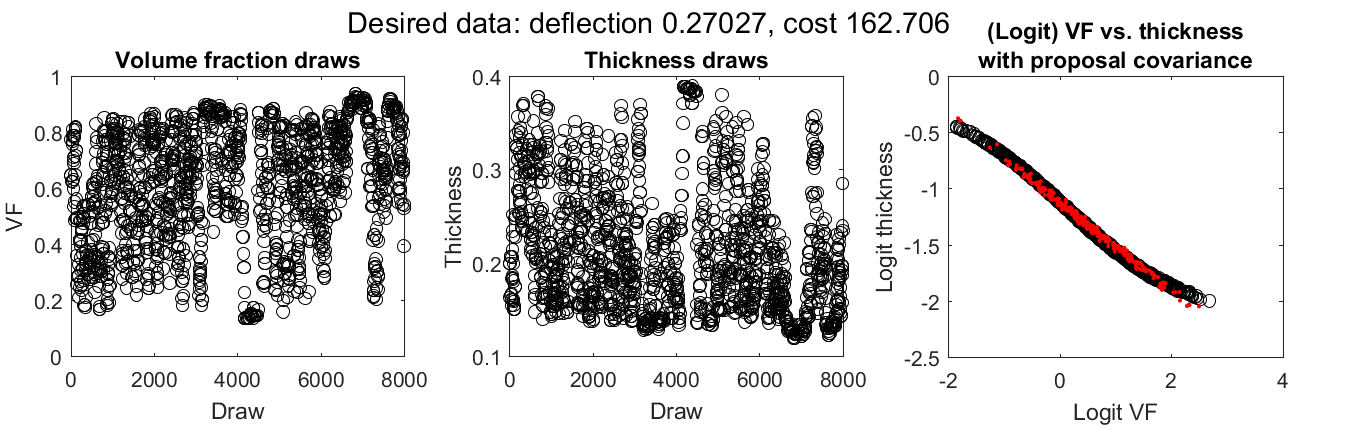
\includegraphics[width=.9\linewidth]{FIG2}
\caption{MCMC results for low deflection and cost (top row) and low deflection with easily achievable cost (bottom row).}
% NOTE: THESE PLOT TITLES ARE WRONG! GOTTA DO THE PLOTS OVER! LOL!
\label{fig:des_data}
\end{figure}

\subsubsection{Identifiability issues}
% Issues arising from the non-identifiability of VF, thickness when cost is relaxed
Blah

\subsection{Non-uniform prior on $\theta$}\label{non-uniform_prior}

\subsubsection{Motivation}

\subsubsection{Implementation}



\subsection{Exponentially distributed desired data}
Blah

\subsubsection{Motivation}
Blah

\subsubsection{Implementation and results}
Blah


\section{Future work}
Blah

\subsection{Alternative means of handling cost}
Blah

\subsubsection{Removing cost from the model}
Blah

\subsubsection{Alternative priors for controlling cost}
Blah

\subsection{Building a desired data response surface}
Blah

\subsection{Implementing Hamiltonian Monte Carlo}
Blah

\subsubsection{Hamiltonian Monte Carlo}
% Background
Blah

\subsubsection{Benefits}
Blah

\subsection{Model discrepancy}
% Include (or investigate the inclusion of) a model discrepancy function
Blah

\section{Conclusion}
% Discussion of the role of computer model validation as a potential methodology for design
Blah












\bibliographystyle{authordate1}
% This style file is a version of the plain.bst style file which I edited myself to add abstract and annotation fields.

\pagebreak

\bibliography{lit_review}

\end{document}